% Version 1.0 by Sajid Mohamed, Geldrop, November 2022
% Thanks - Joost van Pinxten, Joos Buijs
% Use at your own risk.
% Attribution is appreciated

%The main PhD thesis file (compile this one for the full thesis), this file only calls other files for layout and contents, as little as possible should be declared here

% Compiled without errors in Overleaf using 
%---------------------------------------------------------
%This is pdfTeX, Version 3.14159265-2.6-1.40.20 (TeX Live 2019) (preloaded format=pdflatex 2019.12.13)  2 NOV 2022 20:09
%entering extended mode
% \write18 enabled.
% %&-line parsing enabled.
%**main.tex
%(/compile/main.tex
%LaTeX2e <2019-10-01> patch level 3
%----------------------------------------------------------


% \documentclass[draft,b5paper]{book}
\documentclass[b5paper,openany]{book}

%All style, macro and package definitions go here
%NOTICE: NOT USED!!! SEE CONFIG.tex

%
%First the metadata definition
%

% ****************************************************************************************************
% 2. Personal data and user ad-hoc commands
% ****************************************************************************************************
\newcommand{\myTitle}{Multiprocessor Image-Based Control\xspace}
\newcommand{\myFrontpageTitle}{Multiprocessor Image-Based Control: \\Model-Driven Optimisation\xspace}
\title{\myFrontpageTitle}
\newcommand{\myDegree}{Master of Technology\xspace}
\newcommand{\myName}{Sajid Mohamed\xspace}
\author{\myName}
\newcommand{\myProf}{prof.dr.ir. Twan Basten\xspace}
%\newcommand{\myOtherProf}{Put name here\xspace}
\newcommand{\mySupervisor}{dr. Dip Goswami\xspace}
\newcommand{\myFaculty}{Electrical Engineering\xspace}
\newcommand{\myDepartment}{Electronic Systems\xspace}
\newcommand{\myUni}{Eindhoven University of Technology\xspace}
\newcommand{\myLocation}{Eindhoven\xspace}
\newcommand{\myTime}{December 2022\xspace}
\date{} %no date on the title page please
\newcommand{\myVersion}{version 1.0 - Draft}
\newcommand{\myKeywords}{\xspace} % personal data and user ad-hoc commands
% The style file
% Contains settings, macro definitions and package inclusions
%

\usepackage{anyfontsize}
%Personal names etc.
\newcommand{\myTerm}{myTerm} %Example of a term you use often. Prevent typos, use macros!

%Normal text abbreviations
\newcommand{\ie}{i.e.\xspace}
\newcommand{\Ie}{I.e.\xspace}
\newcommand{\eg}{e.g.\xspace}
\newcommand{\Eg}{E.g.\xspace}
\newcommand{\vs}{v.s.\xspace}
\newcommand{\etc}{etc.\xspace}

\newcommand\hmmax{0}
\newcommand\bmmax{0}
% needed to not throw "LaTeX Error: Too many math alphabets used in version normal."

\newcommand{\etal}{et al.\xspace}
\newcommand{\cf}{cf.\xspace}

\usepackage{lmodern}

% footnote without marker, to put a note on the chapters from which papers they arose
\newcommand\blfootnote[1]{%
    \begingroup
    \renewcommand\thefootnote{}\footnote{#1}%
    \addtocounter{footnote}{-1}%
    \endgroup
}
%EXTEND when/if necessary

%This one needs/wants/has to be first
\usepackage[dvipsnames,table]{xcolor} % [dvipsnames]
\definecolor{darkred}{rgb}{0.5,0,0}
\definecolor{darkgreen}{rgb}{0,0.5,0}
\definecolor{darkblue}{rgb}{0,0,0.5}
\definecolor{halfgray}{gray}{0.55} % chapter numbers will be semi transparent .5 .55 .6 .0
\definecolor{webgreen}{rgb}{0,.5,0}
\definecolor{webbrown}{rgb}{.6,0,0}
%define your own colors, also to easily change them all at once

% ********************************************************************
% Setup, finetuning, and useful commands
% ********************************************************************
\newcounter{dummy} % necessary for correct hyperlinks (to index, bib, etc.)
\newlength{\abcd} % for ab..z string length calculation
\providecommand{\mLyX}{L\kern-.1667em\lower.25em\hbox{Y}\kern-.125emX\@}
% ****************************************************************************************************

%---------------------------------------%
% Default fig and table positioning     %
%---------------------------------------%

% From http://tex.stackexchange.com/questions/140568/how-to-set-default-positioning-of-figure-table-document-wide (BY MOI :D)
% and http://tex.stackexchange.com/questions/8351/what-do-makeatletter-and-makeatother-do
\makeatletter
  \providecommand*\setfloatlocations[2]{\@namedef{fps@#1}{#2}}
\makeatother
\setfloatlocations{figure}{b!}
\setfloatlocations{table}{t!}
%\setfloatlocations{subfigure}{t} %does not seem to work the same as adding [t] to begin{subfigure}

%
% Footnote command that has no marker or counter increase
% FROM http://en.wikibooks.org/wiki/LaTeX/Footnotes_and_Margin_Notes
%
\makeatletter
\def\blfootnote{\xdef\@thefnmark{}\@footnotetext}
\makeatother


% ****************************************************************************************************
% 3. Loading some handy packages (alphabetically mainly)
% ****************************************************************************************************

%might be disabled:
\listfiles %include list of used files in .log

\usepackage[fleqn]{amsmath}   % math environments and more by the AMS
\usepackage[paperwidth=17cm,paperheight=24cm, textheight=526pt,marginpar=2cm]{geometry}

% ----------Size of the paper and the margins----------------
%\RequirePackage[paperwidth=17cm, paperheight=24cm, textwidth=12.8cm, textheight = 19.5cm, top=2.5cm, inner=2.2cm, outer=2cm, bottom=2cm]{geometry}

%Use crop package below to place cutlines in the document

%\usepackage[cross,width=17.2cm,height=24.2cm,center]{crop}

\DeclareMathOperator*{\argmin}{arg\,min}
\DeclareMathOperator*{\dom}{dom}
\newcommand{\norm}[1]{\left\lVert#1\right\rVert}
\newcommand{\vect}[1]{\boldsymbol{#1}}

\usepackage{amsthm}
%\newtheorem{definition}{Definition}[chapter]  %We use mainly definitions and number them by chapter
\newtheorem{definition}{Definition}
\newtheorem{proposition}{Proposition}

\usepackage[ruled,vlined,linesnumbered]{algorithm2e}
\usepackage{algorithmic}
\usepackage{amssymb,dsfont}        % f.i. the circular arrows
\usepackage{import} 
\usepackage[dutch,english]{babel} %we need Dutch too, but main text is english so load english last
\usepackage{booktabs}       % for better rules in tables
\usepackage{bm}             % for bold math (eg numbers), still looks kinda ugly
\usepackage{bibentry}       % Inline bibliography entries
\nobibliography*

\usepackage[toc,page]{appendix}
% allow 3-digit page numbers to be rendered properly
\makeatletter
\renewcommand{\@pnumwidth}{2em} 
%\renewcommand{\@tocrmarg}{4em}
\makeatother
\setcounter{tocdepth}{1}
\usepackage{tocvsec2}

\usepackage{calc}           % Calculations, mainly coordinates in TikZ

\usepackage{caption}        % for better captions...
\captionsetup{format=hang,font=small}

\usepackage{cite}           % for neat citations (\eg sorted and abbreviated to 1-20)
\usepackage{comment}        % add a comment environment

\usepackage{datetime}   % time access (mainly for page footer)
\yyyymmdddate
\usepackage{doi}            % provides the \doi{} command that makes DOIs into hyperlinks (not needed if biblatex is enabled I guess)
%\usepackage{dsfont}         % For natural numbers symbol etc.
\usepackage{emptypage}      % Empty pages between chapters!!!!

%Fancy headers!!!
\usepackage{fancyhdr}
\usepackage[Lenny]{fncychap} %We chooose lenny, refer to package doc for more styles
\pagestyle{fancy}
%For more setup see below
\usepackage{mathpazo,tgpagella,tgadventor}
%\linespread{1.05}         % Palladio needs more leading (space between lines)
\usepackage[T1]{fontenc}% T2a for cyrillics (http://tex.stackexchange.com/questions/664/why-should-i-use-usepackaget1fontenc)
\usepackage{fourier}        %For better math font style (tip by Jack van Wijk)
\usepackage{csvsimple}
\usepackage{graphicx}       % Graphics (only text is booooring)
\graphicspath{{./Figures/}} % Which we load from a subdir
\usepackage{array}
%\usepackage[xindy,toc]{glossaries}  
\usepackage[xindy,acronym,nomain,smallcaps,toc]{glossaries} % sorted glossary entries
%\newglossaryentry{ibc}
%{
%    name={IBC},
%    description={image-Based Control},
%    first={\glsentrydesc{ibc} (\glsentrytext{ibc})},
%    plural={IBCs},
%    firstplural={\glsentrydesc{ibc}s (\glsentryplural{ibc})}
%}

\newacronym{adas}{ADAS}{advanced driver assistance system}
\newacronym{aeb}{AEB}{automatic emergency braking}
\newacronym{ai}{AI}{artificial intelligence}
\newacronym{arx}{ARX}{auto-regressive exogenous}
\newacronym{asil}{ASIL}{automotive safety integrity level}
\newacronym{ccd}{CCD}{charge-coupled device}
\newacronym{cmos}{CMOS}{complementary metal–oxide semiconductor}
\newacronym{cnn}{CNN}{convolutional neural network}
\newacronym{cog}{CoG}{centre of gravity}
\newacronym{compsoc}{CompSOC}{composable and predictable multiprocessor system-on-chip}
\newacronym{cps}{CPS}{cyber-physical system}
\newacronym{cpu}{CPU}{central processing unit}
\newacronym{cqlf}{CQLF}{common quadratic Lyapunov function}
\newacronym{dct}{DCT}{discrete cosine transform}
\newacronym{dgpu}{dGPU}{discrete GPU}
\newacronym{dnn}{DNN}{deep neural network}
\newacronym{dram}{DRAM}{dynamic random access memory}
\newacronym{dtmc}{DTMC}{discrete-time Markov chain}
\newacronym{dse}{DSE}{design-space exploration}
\newacronym{ev}{EV}{electric vehicle}
\newacronym{fp}{FP}{failure probability}
\newacronym{fps}{fps}{frames per second}
\newacronym{fsd}{FSD}{full self-driving}
\newacronym{gm}{GM}{gain margin}
\newacronym{gmsl}{GMSL}{gigabit multimedia serial link}
\newacronym{gpu}{GPU}{graphical processing unit}
\newacronym{gpr}{GPR}{generalized precedence relation}
\newacronym{hil}{HiL}{hardware-in-the-loop}
\newacronym{hsdf}{HSDF}{homogeneous synchronous dataflow}
\newacronym{hsdfg}{HSDFG}{homogeneous synchronous dataflow graph}
\newacronym{ibc}{IBC}{image-based control}
\newacronym{igpu}{iGPU}{integrated Pascal GPU}
\newacronym{imacs}{IMACS}{performance evaluation for IMAge-based Control Systems}
\newacronym{io}{I/O}{input/output}
\newacronym{isp}{ISP}{image-signal processing}
\newacronym[plural=LMIs,firstplural=linear matrix inequalities]{lmi}{LMI}{linear matrix inequality}
\newacronym{lkas}{LKAS}{lane-keeping assist system}
\newacronym{lpv}{LPV}{linear parameter-varying}
\newacronym{lqg}{LQG}{linear-quadratic-Gaussian}
\newacronym{lqi}{LQI}{linear-quadratic-integral}
\newacronym{lqr}{LQR}{linear quadratic regulator}
\newacronym{lti}{LTI}{linear time-invariant}
\newacronym{lut}{LUT}{look-up table}
\newacronym{mae}{MAE}{mean absolute error}
\newacronym{mce}{MCE}{maximum control effort}
\newacronym{mimo}{MIMO}{multi-input multi-output}
\newacronym{mjls}{MJLS}{Markovian jump linear system}
\newacronym{moc}{MoC}{model-of-computation}
\newacronym{mpc}{MPC}{model-predictive control}
\newacronym{mpsoc}{MPSoC}{multiprocessor system-on-chip}
\newacronym{mse}{MSE}{mean square error}
\newacronym{nmpc}{NMPC}{nonlinear model-predictive control}
\newacronym{noc}{NoC}{network-on-chip}
\newacronym{npu}{NPU}{neural processing unit}
\newacronym{odt}{ODT}{object detection and tracking}
\newacronym{os}{OS}{operating system}
\newacronym{pm}{PM}{phase margin}
\newacronym{pr}{PR}{perception}
\newacronym{psd}{PSD}{power spectral density}
\newacronym{qoc}{QoC}{quality-of-control}
\newacronym{qp}{QP}{quadratic programming}
\newacronym{rmse}{RMSE}{root mean square error}
\newacronym[plural=RoIs,firstplural=regions-of-interest]{roi}{RoI}{region-of-interest}
\newacronym{sadf}{SADF}{scenario-aware dataflow}
\newacronym{sadfg}{SADFG}{scenario-aware dataflow graph}
\newacronym{sdf}{SDF}{synchronous dataflow}
\newacronym{sdfg}{SDFG}{synchronous dataflow graph}
\newacronym{sil}{SiL}{software-in-the-loop}
\newacronym{siso}{SISO}{single-input single-output}
\newacronym{slc}{SLC}{switched linear control system}
\newacronym{slr}{SLR}{single-lens reflex}
\newacronym{soc}{SoC}{system-on-chip}
\newacronym{spade}{SPADe}{scenario- and platform-aware design}
\newacronym{ssim}{SSIM}{structural similarity}
\newacronym{st}{ST}{settling time}
\newacronym{tcpip}{TCP/IP}{transmission control protocol/internet protocol}
\newacronym{tdm}{TDM}{time-division multiplexing}
\newacronym{wcet}{WCET}{worst-case execution time}
\newacronym{wcrt}{WCRT}{worst-case response time}
\newacronym{xcps}{xCPS}{eXplore Cyber-Physical System}
\newacronym{xil}{XiL}{X-in-the-loop}
\newacronym{zoh}{ZOH}{zero-order hold}

\usepackage{hhline}         % for more specific lines in tables
\usepackage{hyphenat}
%\hyphenation{re-cor-ded re-quire-ments}    % These words were not hyphenated correctly automatically but are now! Extend as necessary
\hyphenation{other-wise}
%\usepackage[latin9]{inputenc}
\usepackage[utf8]{inputenc}  % To prevent '' etc. to appear. 'latin9' is default (I guess) and 'utf8' fails on some 'no-break space' characters which are hard to find...

\usepackage{lastpage}       % To be able to say how many pages we have
\usepackage{lipsum}         % To add some of these fake text we do, you should be able to delete this when your thesis is done! really! Not kidding...
\usepackage{longtable}      % For multi-page tables

\usepackage{makeidx}        % For creating an index which every proper book should have %NOTE: should be loaded before hyperref
%\usepackage{showidx}        % Show index keys in the margin (is not on good terms with hyperref so do NOT enable)
\usepackage{mathtools}      % mathtools builds on and extends amsmath package, used to break long equations over multiple lines in ch. 6
\DeclarePairedDelimiter\ceil{\lceil}{\rceil}
\DeclarePairedDelimiter\floor{\lfloor}{\rfloor}

\newcommand{\asap}[1]{\ensuremath{\underline{#1}}}
\newcommand{\alap}[1]{\ensuremath{\overline{#1}}}

\usepackage{mparhack}       % get marginpar right (known bug)
\usepackage{multirow}       % multiple rows and columns in tables

\usepackage{paralist}       % for inline lists
%\usepackage{pdflscape}      % land scape pages
\usepackage{lscape}
\usepackage{pdfpages}
\usepackage{pifont}         % For the \ding command (used for \tick, \cross, etc.)
\usepackage{placeins}       % Introduces the \FloatBarrier command, but can also be set to never let floats cross section boundaries
\usepackage[draft]{prelim2e}       %Mark prelimenary versions by adding [draft]
\renewcommand{\PrelimWords}{\relax}
\renewcommand{\PrelimText}{\footnotesize[\,\today\ at \currenttime\ -- \pageref{LastPage} pages -- \myVersion\,]} \renewcommand{\PrelimText}{} %Clears the footer all together

\usepackage[inline]{enumitem}
\usepackage{float}
\usepackage{rotating}       % For rotating in tables from Excel (using Excel plug-in)
\usepackage{standalone}     % To make the individual TikZ files also compilable :)

\usepackage{tabularx}       % for vertical alignment in tables
\usepackage[nottoc]{tocbibind}      % We want the bibliography in the TOC please!

%I L-O-V-E TikZ!
% Version 1.0 by Joos Buijs, Eindhoven, August 2014
% Use at your own risk.
% Attribution is appreciated

%
% Dedicated TikZ configuration file to quickly access and set thesis-wide settings and definitions
% This file should also load everything needed to compile particular tikz files stand-alone (eg using TikZEdt)
%

\usepackage{subcaption}     % For subfigures (subfig(ure) packages are deprecated!)

\usepackage{pgfplots}       % Charts in LaTeX, or, even better, in TikZ!!!
\usepgfplotslibrary{colormaps,groupplots,patchplots,statistics} %packages I used
\pgfplotsset{% % NOTE that these worked for me, but are retained as an example
 every axis/.append style={
%      axis lines = left, %set the axis only on the left and bottom sides of the plot      , first $100$ generations
      legend image post style={mark=none},
      cycle list name = linestyles*},
      yticklabel style={/pgf/number format/fixed,/pgf/number format/fixed zerofill,/pgf/number format/precision=3},
      every axis plot /.append style={mark=none},
      every colorbar/.append style={
        colorbar sampled line,
        colorbar horizontal,
  },
%  colormap={joos}{},
  colormap/autumn,
}
\pgfplotsset{compat=1.10}
\pgfplotscreateplotcyclelist{customLineList}{solid,dashed,dashdotted,dashdotdotted,dotted}

\usepackage{pgfplots}
\pgfplotsset{compat=newest}
\usepgfplotslibrary{external} 

%I L-O-V-E TikZ!
\usepackage{tikz}           % The 'normal' TikZ package
\usepackage{tikz-qtree}     % And the QTree-TikZ hybrid package, to make it a lot easier to create process trees
%Also using forest, a TikZ ~extension, see http://www.ctan.org/pkg/forest, mainly produces compacter trees
\usepackage[external]{forest}         % forest can use externalization by adding [external] but it does not listen to the '\tikzsetfigurename{}' command
%\usepackage{forest-qtree}  % prevents compilation :( but would require 'no' code change :D

\usetikzlibrary{calc,decorations.pathreplacing,shapes, fit, intersections, decorations,patterns,arrows,automata,backgrounds,calc,decorations.pathmorphing,decorations.text,decorations.markings,fit,petri,positioning,scopes,shadows,shapes,spy}

\usetikzlibrary{arrows.meta}

%
%
% PGF Plots settings
%
\pgfplotsset{
    every axis/.append style={
        scale only axis,          %instead of scaling text too
    },
    label style={font=\footnotesize},
    legend style={font=\footnotesize}
}
\usepackage{fp}
%
% Define utility macro \customrevertcolormap{X} to revert a color bar
% FROM http://tex.stackexchange.com/a/141338/27955
%
\makeatletter
\def\customrevertcolormap#1{%
    \pgfplotsarraycopy{pgfpl@cm@#1}\to{custom@COPY}%
    \c@pgf@counta=0
    \c@pgf@countb=\pgfplotsarraysizeof{custom@COPY}\relax
    \c@pgf@countd=\c@pgf@countb
    \advance\c@pgf@countd by-1 %
    \pgfutil@loop
    \ifnum\c@pgf@counta<\c@pgf@countb
        \pgfplotsarrayselect{\c@pgf@counta}\of{custom@COPY}\to\pgfplots@loc@TMPa
        \pgfplotsarrayletentry\c@pgf@countd\of{pgfpl@cm@#1}=\pgfplots@loc@TMPa
        \advance\c@pgf@counta by1 %
        \advance\c@pgf@countd by-1 %
    \pgfutil@repeat
%\pgfplots@colormap@showdebuginfofor{#1}%
}%
\makeatother

\usepackage[colorinlistoftodos,backgroundcolor=white,linecolor=gray]{todonotes}  %More advanced todos, default todo has no color
%And different predefined todos (change as you see fit)
%\newcommand{\RW}[1][]{\todo[color=green!40]{RW: #1}}
\newcommand{\atProf}[1]{\todo[color=blue!40]{@W: #1}}
\newcommand{\status}[1]{\todo[color=purple!40]{STATUS: #1}}

\newcommand{\should}[1]{\todo[color=red!40]{#1}}  % 'must do' todos
\newcommand{\could}[1]{\todo[color=orange!40]{#1}}   % easy improvement todos
\newcommand{\would}[1]{\todo[color=yellow!40]{#1}}   % suggestions
\newcommand{\may}[1]{\todo{#1}}     % maybe...

\newcommand{\forFinal}[1]{\todo[color=brown!40]{#1}} %Action points before final version is created

\usepackage{todonotes}
\newif\iftodoused
\newcommand{\todosajid}[2][]
{\iftodoused\todo[inline, color=green!20, #1]{\small\textbf{Sajid: }#2}\fi}
\newcommand{\todotwan}[2][]
{\iftodoused\todo[inline, color=pink!20, #1]{\small\textbf{Twan: }#2}\fi}
\newcommand{\tododip}[2][]
{\iftodoused\todo[inline, color=orange!20, #1]{\small\textbf{Dip: }#2}\fi}

\renewcommand{\arraystretch}{1.2}
%%%%%TO TURN TODO NOTES ON/OFF ::::
%
\renewcommand{\todo}[2][]{}

\usepackage{wasysym}        % For the correct sized circle inside the BPMN gateways...

\usepackage{xspace}         %To add space to command definitions


%\usepackage{fixltx2e} % fixes some LaTeX stuff
\usepackage{textcomp} % fix warning with missing font shapes

% PDFLaTeX, hyperreferences and citation backreferences
% ****************************************************************************************************
% PDFLaTeX
% ocgcolorlinks : ensures that colored links are printed as black (when supported by PDF viewer!) (from http://tex.stackexchange.com/questions/4425/is-there-a-way-to-have-coloured-hyperref-hyperlinks-in-the-pdf-but-have-them-pr)
% NOTE: ocgcolorlinks does not seem to work for me, so made all links black!
\PassOptionsToPackage{hidelinks,pdftex,hyperfootnotes=false,pdfpagelabels,ocgcolorlinks,pdfpagelayout=TwoPageRight,utf8}{hyperref}
\PassOptionsToPackage{hyphens,sloppy}{url}
\RequirePackage{hyperref}
\makeatletter
\g@addto@macro{\UrlBreaks}{\UrlOrds}
\makeatother
\pdfcatalog{/PageLayout /TwoPageRight}
% ********************************************************************
% Setup the style of the backrefs from the bibliography
% ********************************************************************

% disable when using biblatex!!!
\newcommand{\backrefnotcitedstring}{\relax}%(Not cited.)
\newcommand{\backrefcitedsinglestring}[1]{(Cited on page~#1.)}
\newcommand{\backrefcitedmultistring}[1]{(Cited on pages~#1.)}
		\PassOptionsToPackage{hyperpageref}{backref}
\usepackage[hyperpageref]{backref} % to be loaded after hyperref package
   \renewcommand{\backreftwosep}{ and~} % separate 2 pages
   \renewcommand{\backreflastsep}{, and~} % separate last of longer list
   \renewcommand*{\backref}[1]{}  % disable standard
   \renewcommand*{\backrefalt}[4]{% detailed backref
      \ifcase #1 %
         \backrefnotcitedstring%
      \or%
         \backrefcitedsinglestring{#2}%
      \else%
         \backrefcitedmultistring{#2}%
      \fi}%

% ********************************************************************
% Hyperreferences
% ********************************************************************
\hypersetup{%
%    draft,	% = no hyperlinking at all (useful in b/w printouts)
    colorlinks=false,
%     hidelinks=true,
%    colorlinks=true,
    linktocpage=true, pdfstartpage=3, pdfstartview=FitV,%
    % uncomment the following line if you want to have black links (\eg, for printing)
    colorlinks=false, linktocpage=false, pdfborder={0 0 0}, pdfstartpage=3, pdfstartview=FitV,%
    linktoc=all, %make whole line in TOC clickable
    breaklinks=true, pdfpagemode=UseNone, pageanchor=true, pdfpagemode=UseOutlines,%
    plainpages=false, bookmarksnumbered, bookmarksopen=true, bookmarksopenlevel=1,%
    hypertexnames=true, pdfhighlight=/O,%nesting=true,%frenchlinks,%
    urlcolor=webbrown, linkcolor=RoyalBlue, citecolor=webgreen, %pagecolor=RoyalBlue,%
    %urlcolor=Black, linkcolor=Black, citecolor=Black, %pagecolor=Black,%
    pdftitle={\myTitle},%
    pdfauthor={\textcopyright\ \myName, \myUni, \myFaculty},%
    pdfsubject={},%
    pdfkeywords={\myKeywords},%
    pdfcreator={pdfLaTeX},%
    pdfproducer={LaTeX with hyperref}
}

\usepackage[percent]{overpic}
%Correct autoref names
\makeatletter
\addto\extrasenglish{
\renewcommand*{\figureautorefname}{Figure}%
\renewcommand*{\tableautorefname}{Table}%
\renewcommand*{\partautorefname}{Part}%
\renewcommand*{\chapterautorefname}{Chapter}%
\renewcommand*{\sectionautorefname}{Section}%
\renewcommand*{\subsectionautorefname}{Section}%
\renewcommand*{\subsubsectionautorefname}{Section}% 	
\providecommand{\subfigureautorefname}{\figureautorefname}%
\providecommand{\definitionautorefname}{Definition} % It's that easy!: http://tex.stackexchange.com/questions/46258/how-to-get-correct-autoref-for-theorems
}
%\RequirePackage[l2tabu, orthodox]{nag}
\makeatother

% for the chapter blocks on the sides
\usepackage{tikzpagenodes}
\usepackage{totcount}
\usepackage[contents={},opacity=1,scale=1,color=white]{background}
%
% Fancy Headers!!!
%

%Lesli Lamports LaTeX book style headers, from fancyhdr manual page 13
\fancyheadoffset[LE,RO]{\marginparsep+\marginparwidth}
\renewcommand{\chaptermark}[1]{\markboth{#1}{}}
\renewcommand{\sectionmark}[1]{\markright{\thesection\ #1}}
\fancyhf{}
\fancyhead[LE,RO]{\bfseries\thepage}
\fancyhead[LO]{\bfseries\rightmark}
\fancyhead[RE]{\bfseries\leftmark}
\fancypagestyle{plain}{%
 \fancyhead{} % get rid of headers
 \renewcommand{\headrulewidth}{0pt} % and the line
 \renewcommand{\chaptermark}[1]{\markboth{}}
}
% Creates a page footer with page number at the centre
\fancypagestyle{plain}{%
\fancyhf{}% clear all header and footer fields
\fancyfoot[C]{\textbf{\thepage}} % except the center
\renewcommand{\headrulewidth}{0pt}%
\renewcommand{\footrulewidth}{0pt}%
\renewcommand{\footskip}{50pt}
}

\newif\ifwebversion
\webversiontrue
%\usepackage{showframe}
\ifwebversion
\else
\usepackage[width=17.6cm,height=24.6cm,cam,center]{crop}
\fi

\usepackage{background}

\newif\ifMaterial

\newlength\LabelSize
\setlength\LabelSize{1cm}

\AtBeginDocument{%
    \regtotcounter{chapter}%
}
\newcommand\AddChapterBoxes{%
    \Materialtrue
    \AddEverypageHook{%
        \ifx\@chapapp\appendixname%
        \relax%
        \else%
        \ifMaterial%
        \ifodd\value{page}%
        \backgroundsetup{
            angle=0,
            position={current page.east|-current page text area.north east},
            vshift=-30-(\thechapter-1)*1.5*\LabelSize,
            hshift=-10,
            contents={%
                \tikz\node[ch label, inner xsep=\LabelSize/2] {\hspace*{-\LabelSize}\bfseries{\thechapter}};
            }%
        }%
        \else%
        \backgroundsetup{
            angle=0,
            position={current page.west|-current page text area.north west},
            vshift=-30-(\thechapter-1)*1.5*\LabelSize,
            hshift=10,
            contents={%
                \tikz\node[ch label, inner xsep=\LabelSize/2]{\color{white}\bfseries{\thechapter}\hspace*{-\LabelSize}}; % without the \color{white}, the position is not correct yet! not centered to the left half of the block for some reason...
            }%
        }%
        \fi%
        \BgMaterial%
        \else\relax\fi%
        \fi%
    }%
}

\tikzset{
    ch label/.style={fill=black,anchor=west,text width=\LabelSize, align=center,minimum height=\LabelSize,minimum width=\LabelSize*2,inner sep=+0pt,rounded corners=0.25cm,text=white,font=\sffamily\fontsize{15pt}{0pt}\selectfont},
}

\makeatletter

\ChNumVar{\fontsize{36}{80}\usefont{OT1}{pag}{m}{n}\selectfont}
\renewcommand{\DOCH}{%
%Horizontal line left top
    \settowidth{\px}{\CNV\FmN{\@chapapp}}
    \addtolength{\px}{2pt}

%Horizontal line top
    \setlength{\py}{0pt}
    \setlength{\mylen}{0pt}

    \settowidth{\pxx}{\CNoV\thechapter}
    \addtolength{\pxx}{-1pt}
    \par
    \parbox[b]{\textwidth}{%
    \raggedright%
    \color{red}
    \CNoV
%\FmN{\@chapapp}
    \hskip1pt%
    \thechapter%
    \hskip1pt%
    \color{black}
    \rule{\RW}{\pyy}\par\nobreak%
    \vskip -\baselineskip%
    \vskip -\pyy%
    \hskip \mylen%
    \vskip \pyy}%
    \vskip 20\p@}

\renewcommand{\DOTI}[1]{%
    \raggedright
    \CTV\FmTi{#1}\par\nobreak
    \vskip 40\p@}

  \renewcommand{\DOTIS}[1]{%
    \raggedright
    \CTV\FmTi{#1}\par\nobreak
    \vskip 40\p@}

\makeatother

\usepackage[explicit]{titlesec}
\usepackage{nextpage}
\usepackage{ifoddpage}

\usepackage{thm-restate}

\usepackage{etoolbox}

\usepackage[shortcuts]{extdash}
\makeglossaries
\usepackage{hyperref}
%\usepackage{cleverref}
\usepackage{wrapfig}
\usepackage{threeparttable}
\usepackage{textcomp}
\usepackage{setspace}
\usepackage{stackengine}
\newcommand\textsub[1]{\stackengine{-.5ex}{}{\scriptsize#1}{O}{l}{F}{F}{L}}

%%% Infrastructure    
\makeatletter
\newcommand{\refcheckize}[1]{%
  \expandafter\let\csname @@\string#1\endcsname#1%
  \expandafter\DeclareRobustCommand\csname relax\string#1\endcsname[1]{%
    \csname @@\string#1\endcsname{##1}\@for\@temp:=##1\do{\wrtusdrf{\@temp}\wrtusdrf{{\@temp}}}}%
  \expandafter\let\expandafter#1\csname relax\string#1\endcsname
}
\newcommand{\refcheckizetwo}[1]{%
  \expandafter\let\csname @@\string#1\endcsname#1%
  \expandafter\DeclareRobustCommand\csname relax\string#1\endcsname[2]{%
    \csname @@\string#1\endcsname{##1}{##2}\wrtusdrf{##1}\wrtusdrf{{##1}}\wrtusdrf{##2}\wrtusdrf{{##2}}}%
  \expandafter\let\expandafter#1\csname relax\string#1\endcsname
}
\makeatother

\refcheckize{\cref}
\refcheckize{\Cref}
%\refcheckize{\eqref}
\refcheckizetwo{\crefrange}
\refcheckizetwo{\Crefrange}

%********************************************************
%% Sections
% \newtheorem{algorithm}[theorem]{Algorithm}
\newtheorem{theorem}{Theorem}[section]
\newtheorem{claim}[theorem]{Claim}
\newtheorem{comments}[theorem]{Comments}
\newtheorem{construction}[theorem]{Construction}
\newtheorem{corollary}[theorem]{Corollary}
%\newtheorem{definition}{Definition}
% \newtheorem{definition}[theorem]{\textbf{Definition}}
%\newtheorem{definition}{Definition}[chapter]  %We use mainly definitions and number them by chapter
\newtheorem{example}[theorem]{Example}
\newtheorem{lemma}[theorem]{Lemma}
\newtheorem{problem}[theorem]{Problem}
%\newtheorem{proposition}{Proposition}
% \newtheorem{proposition}[theorem]{Proposition}
\newtheorem{remark}[theorem]{Remark}
\newtheorem{xca}[theorem]{Exercise}

%% user commands

%% Symbols
\newcommand{\argmax}{\textrm{arg}\max}
\newcommand{\B}{{\mathbb B}}
\newcommand{\Ce}{{\mathbb C}}
\newcommand{\Expectation}[1]{\ensuremath{\mathds{E}[#1]}}
\newcommand{\ExpectationBig}[1]{\ensuremath{\mathds{E}\Big[#1\Big]}}
\newcommand{\F}{{\mathbb{F}}}
\newcommand{\Inv}{{\mathrm{Inv}}}
\newcommand{\N}{{\mathbb{N}}}
\newcommand{\Natural}{\mathbb{N}}
\newcommand{\Next}{{\mathrm{Next}}}
\newcommand{\Pre}{\mathrm{Pre}}
\newcommand{\Post}{\textrm{Post}}
\newcommand{\Q}{{\mathbb{Q}}}
\newcommand{\R}{{\mathbb{R}}}
\renewcommand{\Re}{{\mathbb{R}}}
\newcommand{\Reach}{{\mathrm{Reach}}}
\newcommand{\Real}{\mathbb{R}}
\newcommand{\reals}{\ensuremath{(\R, <, +, -, \cdot, 0,1)}}
\newcommand{\T}{{\mathbb T}}
\newcommand{\UP}{\textrm{UP}}
\newcommand{\X}{{\mathbf{X}}}
\newcommand{\Ze}{{\mathbb Z}}

%% Miscellaneous
\newcommand{\ea}{{\it et al }}
\newcommand{\D}{\displaystyle}
\newcommand{\kr}{\textrm{ker}}
\renewcommand{\dim}{\mathrm{dim}}
\newcommand{\lie}{\mathrm{Lie}}
\newcommand{\cl}{\mathrm{cl}}
\newcommand{\inte}{\mathrm{int}}
\newcommand{\E}{\mathrm{End}}

%% Dataflow
\newcommand{\actorET}{e}
\newcommand{\Actors}{\mathcal{A}}
\newcommand{\anActor}{a}
\newcommand{\atask}{t}
\newcommand{\binding}{\mathcal{B}}
\newcommand{\bindingAwareSDFG}[1]{\SDFG_{#1}^b}
\newcommand{\bufferSize}{b}
\newcommand{\Channels}{\mathcal{C}}
\newcommand{\concurrencyVector}{\varphi}
\newcommand{\Configuration}{\chi}
\newcommand{\detector}{\mathcal{D}}
\newcommand{\Edges}{\mathcal{E}}
\newcommand{\FnScenarioToOutput}{m}
\newcommand{\FnThroughput}{\nu}
\newcommand{\FnWtoScenarios}{f}
\newcommand{\fsmInitialState}{q_0}
\newcommand{\fsmLabelling}{\nu}
\newcommand{\fsmsadf}{\mathcal{F}}
\newcommand{\fsmStates}{Q}
\newcommand{\fsmTransition}{\delta}
\newcommand{\initialTokens}{i}
\newcommand{\latency}{l}
\newcommand{\latencies}{\mathcal{L}}
\newcommand{\Mapping}{\Gamma}
\newcommand{\mapping}{\gamma}
\newcommand{\maxplusLambda}[2]{\bm{\gamma_{#1}^{#2}}}
\newcommand{\maxplusMatrix}{\bm{G}}
\newcommand{\maxplusMatrixOutput}{\bm{H}}
\newcommand{\parallelisationVector}{\varphi}
\newcommand{\rate}{\mathcal{R}}
\newcommand{\ratesSDFG}{r}
\newcommand{\rateY}{z}
\newcommand{\repetitionVector}{\rho}
\newcommand{\replicationVector}{\varphi}
\newcommand{\Scenarios}{\Sigma}
\newcommand{\scenario}{s}
\newcommand{\SDFG}{\mathcal{G}}
\newcommand{\Tasks}{\mathrm{T}}
\newcommand{\tileConnections}{\mathcal{T_C}}
\newcommand{\tileLatency}{L}
\newcommand{\tiles}{\mathcal{T}}
\newcommand{\transformCamera}{Cam}
\newcommand{\transformFixTiming}{ReT}
\newcommand{\transformIFD}{\mathit{ifd}}
\newcommand{\transformReplicate}{RepP}
\newcommand{\transformParallel}{RepA}
\newcommand{\transformPeriod}{Per}
\newcommand{\transformSequential}{Pipe}
\newcommand{\transformWorkload}{Wld}

%% Platform-related
\newcommand{\comm}{CA}
\newcommand{\fd}{f_d}
\newcommand{\fps}{\mathit{fps}}
\newcommand{\fh}{f_h}
\newcommand{\memory}{M}
\newcommand{\nw}{NI}
\newcommand{\processor}{P}
\newcommand{\TsBCET}{\actorET_{ts}^{bc}}
\newcommand{\TsWCET}{\actorET_{ts}^{wc}}

%% SPADe CORE
\newcommand\aWorkload{w}
\newcommand\numCores{n_c}
\newcommand\numCoresAvailable{n_c^{avl}}
\newcommand\numCoresParallel{n_c^{//}}
\newcommand\numPipes{p}
\newcommand\maxCores{n_c^{max}}
\newcommand\setW{W}
\newcommand\sysScenario{\scenario_s}
\newcommand\workloadScenario{\scenario_i}

%% SPADe-related miscellaneous
\newcommand\anApplication{a}
\newcommand\Applications{\mathcal{A}}
\newcommand\ECU{\psi}
\newcommand\ECUTaskPriority{\taskPriority}
\newcommand\pathsTG{\Pi}
\newcommand\prodTime{\bm{p}}
\newcommand\taskBCET{\actorET^{bc}}
\newcommand\taskDeadline{d}
\newcommand\taskJitter{j}
\newcommand\taskOffset{o}
\newcommand\taskPeriod{pd}
\newcommand\taskPriority{\mathcal{P}}
\newcommand\taskWCET{\actorET^{wc}}
\newcommand\SF{\mathcal{B}}
\newcommand\messagem{m}
\newcommand\messageSize{size}
\newcommand\commBus{\mathcal{B}}
\newcommand\commMapping{\Gamma^m}
\newcommand\platformConnections{\zeta}

%% SPADe tasks
\newcommand{\taskS}{S}
\newcommand{\taskC}{C}
\newcommand{\taskA}{A}
\newcommand{\taskISP}{I}
\newcommand{\taskRoID}{D}
\newcommand{\taskRoIP}{P}
\newcommand{\taskRoIM}{M}

%% Control state-space 
\newcommand{\Adyn}{A_{d}}
\newcommand{\Bdyn}{B_{d}}
\newcommand{\Cdyn}{C_{d}}
\newcommand{\Ddyn}{D_{d}}
\newcommand{\Acont}{A_{c}}
\newcommand{\Bcont}{B_{c}}
\newcommand{\Ccont}{C_{c}}
\newcommand{\Dcont}{D_{c}}
\newcommand{\Kgain}{K}
\newcommand{\Fgain}{F}
\newcommand{\Aaugi}{A_{aug,\workloadScenario}}
\newcommand{\Baugi}{B_{aug,\workloadScenario}}
\newcommand{\Caug}{C_{aug}}
\newcommand{\Aaugs}{A_{aug,\sysScenario}}
\newcommand{\Baugs}{B_{aug,\sysScenario}}

%% Control-related
\newcommand\Controllers{\mathcal{CTRL}}
\newcommand\FnWtoTau{\lambda}
\newcommand\MSE{MSE}
\newcommand\qoc{\Phi}
\newcommand\controlRef{r_{ref}}
\newcommand\SwitchRealisable{\mathcal{RSM}}
\newcommand\SwitchModes{\mathcal{SM}}
\newcommand\Tau{\mathcal{T}}
\newcommand\yL{{y_L}}

%% algorithm-related
\newcommand{\nosemic}{\renewcommand{\@endalgocfline}{\relax}}% Drop semi-colon ;
\newcommand{\dosemic}{\renewcommand{\@endalgocfline}{\algocf@endline}}% Reinstate semi-colon ;
\newcommand{\pushline}{\Indp}% Indent
\newcommand{\popline}{\Indm}% Undent
\let\oldnl\nl% Store \nl in \oldnl
\newcommand{\nonl}{\renewcommand{\nl}{\let\nl\oldnl}}% Remove line number for one line


%% Others
\newcommand{\ActivationType}[1]{\xrightarrow{#1}}
\newcommand{\ArrivalFunction}[2]{\alpha_{#1}^{#2}}
\newcommand\CauseEffectChain{\Pi}
\newcommand{\ServiceFunction}[2]{\beta_{#1}^{#2}}

%% CDC 2019
%********************************************************
\usepackage{subcaption}
\usepackage{cleveref}
\captionsetup[subfigure]{subrefformat=simple,labelformat=simple}
\renewcommand\thesubfigure{(\alph{subfigure})}

\renewcommand{\dim}{\mathrm{dim}}
\newcommand{\q}{\mathsf{q}}
\newcommand{\p}{\mathsf{p}}
\newcommand{\ra}{\rightarrow}
\newcommand{\sigalg}{\mathcal{F}}
\newcommand{\filtration}{\mathds{F}}
\newcommand{\insertref}{\textcolor{red}{[ref]}}
\newcommand{\ul}{\underline}
\newcommand{\ol}{\overline}
\newcommand{\Let}{:=}
\newcommand{\EE}{\mathds{E}}
\newcommand{\PP}{\mathds{P}}
\newcommand{\traj}[3]{#1_{#2#3}}
\newcommand{\sstf}{ \textrm{SStF-}\textrm{M}_{2}}
\newcommand{\ssf}{ \textrm{SSF-}\textrm{M}_{2}}
\newcommand{\infgen}[1]{\mathcal{L}#1}
\newcommand{\define}{\coloneqq}
\newcommand{\Falgebra}{\ensuremath{\mathcal{F}}}
\newcommand{\Pprob}{\ensuremath{\mathds{P}}}
\newcommand{\ExtInputMap}{\ensuremath{\mathcal{U}}}
\newcommand{\IntInputMap}{\ensuremath{\mathcal{W}}}
\newcommand{\horizontalline}{\noindent\makebox[\linewidth]{\rule{\paperwidth}{0.4pt}}}
\newcommand{\horizontalEqSep}{\noindent\rule{18cm}{0.4pt}}
\newcommand{\expo}{\mathsf{e}}
\newcommand{\diff}{\mathsf{d}}
\newcommand{\defeq}{\vcentcolon=}
\def\MZ#1{{\textcolor{red}{ {\bf MZ:} #1}}}
\newcommand{\kinf}{$\mathcal{K}_{\infty}$}

\def\ve{\varepsilon}
\def\ts{\widetilde{S}}
\def\q{\mathsf q}

%Generate index 
\makeindex

\tikzset{
    chapter pic/.style={
        inner sep=0pt,
        outer sep=0pt,
        opacity=.5
    },
    chapter name/.style={
        xshift=-25mm,
        yshift=30mm,
        font=\sffamily\bfseries\Huge,
        text=black},
    chapter number/.style={
        white,
        scale=15,
        yshift=-1mm
    },
    chapter text/.style={
        fill=black!80!black,
        text=white,
        font=\Huge\bfseries,
        inner ysep=12pt,
        inner xsep=20pt,
        rounded rectangle,
        xshift=-20mm,
        yshift=7.5mm
    },
}


\begin{document}

%% uncomment below to include the cover page
%\ifwebversion
%\includepdf{cover-full.pdf}
%\fi

%\begin{comment} %uncomment to avoid the graphics on Chapter first pages
\definecolor{chapopcolor}{cmyk}{0.95,0.75,0.5,0.7} % specific for my thesis
\definecolor{covergold}{cmyk}{0.2,0.3,0.55,0.05} % specific for my thesis
\makeatletter
\titleformat{name=\chapter}{}{}{0pt}{
    \Materialfalse%
    \thispagestyle{empty}%
\checkoddpage%
\ifoddpage%
    \clearpage%\cleartoevenpage%
\fi
    \thispagestyle{empty}%
    \begin{tikzpicture}[overlay,remember picture]%
    \node [anchor=south west, chapter pic,xshift=-3mm,yshift=-3mm] at (current page.south west) {
\includegraphics{chapter-pages-bleed.pdf}};
    \fill[chapopcolor,opacity=0.75] ([xshift=-5mm, yshift=-5mm] current page.south west) rectangle ([xshift=5mm, yshift=5mm] current page.north east);
    \fill[chapopcolor,opacity=.75] ([yshift=-30mm] current page.west) rectangle (current page.south east);
     \foreach \x in {-3,...,14}
        \foreach \y in {-3,...,21} 
        {
            \pgfmathtruncatemacro{\odd}{mod(\y,2)}    
            %    {\pgfmathtruncatemacro{\label}{\x - 5 *  \y +21}
            \pgfmathrandominteger{\alea}{0}{4}
            \node[covergold,circle,fill,inner sep=0em,minimum size=\alea*0.5em] (\x\y) at (1*\x + \odd*0.5,-1*\y) {}; 
        }
        \node [chapter number] at (current page.center) {{\fontfamily{qag}\selectfont\bfseries\Huge\thechapter}};
    \end{tikzpicture}
    \clearpage
    \thispagestyle{plain}
    \begin{tikzpicture}[overlay,remember picture]
    \node [anchor=south east, chapter pic,xshift=3mm,yshift=-3mm] at (current page.south east) {
\includegraphics{chapter-pages-bleed.pdf}};
    \end{tikzpicture}
    \vspace*{10mm}
    \begin{flushright}
        {\fontfamily{qag}\selectfont\bfseries\huge#1}
    \end{flushright}
    \vspace*{10mm}
    \afterpage{}       
}
\titleformat{name=\chapter,numberless}{}{}{0pt}{
    \Materialfalse
    %\clearpage
    %\thispagestyle{plain}
    \begin{tikzpicture}[overlay,remember picture]
    \node [anchor=south west, chapter pic,xshift=-3mm,yshift=-3mm] at (current page.south west) {
\includegraphics{chapter-pages-bleed.pdf}};
    \end{tikzpicture}
    \thispagestyle{plain}
    \begin{tikzpicture}[overlay,remember picture]
    \node [anchor=south east, chapter pic,xshift=3mm,yshift=-3mm] at (current page.south east) {
\includegraphics{chapter-pages-bleed.pdf}};
    \end{tikzpicture}
    \vspace*{10mm}
    \begin{flushright}
        {\fontfamily{qag}\selectfont\bfseries\huge#1}
    \end{flushright}
    \vspace*{10mm}
}
\makeatother
\titlespacing*{\chapter}{0pt}{0pt}{0pt}    

\frontmatter
%\end{comment} %uncomment to avoid the graphics on Chapter first pages

\pagenumbering{roman}
% Frontmatter
%
% THIS FILE IS EINDHOVEN UNIVERSITY OF TECHNOLOGY SPECIFIC!!!
%

\thispagestyle{empty}
\noindent

\begin{center}

\huge % or \Huge

%\vspace{5em}

\myFrontpageTitle

\vspace{3em}

\Large
PROEFSCHRIFT

\vspace{3em}

ter verkrijging van de graad van doctor aan de Technische Universiteit Eindhoven, op gezag van de rector magnificus prof.dr.ir. F.P.T. Baaijens, 
voor een commissie aangewezen door het College voor Promoties, in het openbaar te verdedigen op
\\dinsdag 20 december 2022 om 16:00 uur


\vspace{3em}

%\large
door

%\Large
\vspace{3em}

Sajid Mohamed

\vspace{3em}

%\large
geboren te Trivandrum, Kerala, India

\end{center}


\newpage
\thispagestyle{empty}
\normalsize

\noindent
Dit proefschrift is goedgekeurd door de promotoren en de samenstelling van de promotiecommissie is als volgt: 

\vspace{1em}
\noindent
\begin{tabular}{ll}
Voorzitter:     & prof.dr.ir. M. Matters-Kammerer  \\
Promotor:    & \myProf  \\
Copromotor:    & \mySupervisor   \\
Promotie-  &  \\ 
commissieleden:
& prof.dr.ir. T. Basten  \\
                & dr. D. Goswami   \\
                & prof.dr. K.G.W. Goossens    \\ 
                & prof.dr.ir. J.P.M. Voeten    \\  
                & prof.dr. A. Jantsch \hspace{4em}  \  (Technische Universit\"at Wien) \\
                & prof.dr.sc. S. Chakraborty\hspace{1em} (UNC Chapel Hill) \\               
\end{tabular}

\vfill
\noindent \emph{Het onderzoek dat in dit proefschrift wordt beschreven is uitgevoerd in overeenstemming met de TU/e Gedragscode Wetenschapsbeoefening.}
%*******************************************************
% Titlepage
%*******************************************************
\thispagestyle{empty}
\maketitle 
%Titlepage backside
\thispagestyle{empty}
\noindent
\begin{tabular}{p{104mm}}

\noindent
The work described in this thesis was carried out at the Eindhoven University of Technology. 
This work is part of the research program "oCPS" funded from the European Union's Horizon 2020 Framework Programme for Research and Innovation under grant agreement No. 674875.
\\[6mm]

\begin{tabular}{ccc}
    
\includegraphics[width=3cm]{Figures/TUe-logo-scarlet-L.png}&  
     
\includegraphics[scale=0.3]{Figures/European_Commission.jpg}&
    
\includegraphics[scale=0.2]{Figures/oCPSlogo.jpg}
    
\end{tabular}

\\[6mm]

\end{tabular}

\vfill
\noindent
\begin{tabular}{p{104mm}}


Copyright \copyright{} 2022, \myName. \\
All rights reserved. 
Reproduction in part or in whole is prohibited \\ without the written consent of the copyright owner.\\
Typeset in LaTeX. Source: \href{https://github.com/sajid-mohamed/sajidPhDThesis}{github.com/sajid-mohamed/sajidPhDThesis} 
\\[2mm]
Cover photo from shutterstock. \\Cover design by Vincent van Zandvoord (Buro Vormvast).
\\[2mm]
Printed by Proefschriftmaken, The Netherlands
\\[2mm]
A catalogue record is available from the \\Eindhoven University of Technology Library. \\[2mm]
ISBN 978-90-386-5580-2

\end{tabular}
\cleardoublepage

%*******************************************************
% Dedication
%*******************************************************
\thispagestyle{empty}
%\clearpage

\par\vspace*{.15\textheight}{\centering Dedicated to my parents (\emph{Umma, Vappa}) and my wife (Jemshi).\par}

\par\vspace*{.35\textheight}{\centering In the loving memory of my grandfathers.\\Your love, encouragement and prayers will always stay with me. \par}

\cleardoublepage
\patchcmd{\chapter}{\cleardoublepage}{\relax}{}{}
\patchcmd{\chapter}{\clearpage}{\relax}{}{}
% Short English abstract here
\phantomsection
\chapter*{Summary}
\begin{center}
    \bfseries\large\myFrontpageTitle
\end{center}
\addcontentsline{toc}{chapter}{Summary}
\thispagestyle{empty}

\glsresetall
\hyphenation{ana-lysis}

\begin{sloppypar}
Over the last years, cameras have become an integral component of modern cyber-physical systems due to their versatility, relatively low cost and multi-functionality. Camera sensors form the backbone of modern applications like \glspl{adas}, visual servoing, telerobotics, autonomous systems, electron microscopes, surveillance and augmented reality. \Gls{ibc} systems refer to a class of data-intensive feedback control systems whose feedback is provided by the camera sensor(s). \Gls{ibc} systems have become popular with the advent of efficient image-processing algorithms, low-cost \gls{cmos} cameras with high resolution and embedded multiprocessor computing platforms with high performance. The combination of the camera sensor(s) and image-processing algorithms can detect a rich set of features in an image. These features help to compute the states of the \gls{ibc} system, such as relative position, distance, or depth, and support tracking of the object-of-interest. Modern industrial compute platforms offer high performance by allowing parallel and pipelined execution of tasks on their multiprocessors.
\end{sloppypar}
The challenge, however, is that the image-processing algorithms are compute-intensive and result in an inherent relatively long sensing delay. State-of-the-art design methods do not fully exploit the \gls{ibc} system characteristics and advantages of the multiprocessor platforms for optimising the sensing delay. The sensing delay of an \gls{ibc} system is moreover variable with a significant degree of variation between the best-case and worst-case delay due to application-specific image-processing workload variations and the impact of platform resources. A long variable sensing delay degrades system performance and stability. A tight predictable sensing delay is required to optimise the \gls{ibc} system performance and to guarantee the stability of the \gls{ibc} system. Analytical computation of sensing delay is often pessimistic due to image-dependent workload variations or challenging platform timing analysis. Therefore, this thesis explores techniques to cope with the long variable sensing delay by considering application-specific \gls{ibc} system characteristics and exploiting the benefits of the multiprocessor platforms. Effectively handling the long variable sensing delay helps to optimise \gls{ibc} system performance while guaranteeing \gls{ibc} system stability.

First, this thesis presents the model-driven \gls{spade} flow for \gls{ibc} systems modelling, analysis, design and implementation.  The \gls{spade} flow expressly targets \gls{mpsoc} platforms. The thesis develops the \gls{spade} flow with a focus on the \gls{compsoc} platform. The thesis further presents an adaptation of the \gls{spade} flow for modern industrial platforms – NVIDIA Drive PX2 and NVIDIA AGX Xavier, which are closed-source and difficult to predict. The \gls{spade} flow is validated using the \gls{imacs} framework developed as part of this thesis.
The \gls{spade} flow is explained incrementally in this thesis starting with the platform-specific aspects and later showing how the application-specific aspects are integrated.   

The platform-specific aspects explored in this thesis are application parallelism and pipelining of the control loop. First, we examine the case of application parallelism with no pipelining allowed for the control loop. A \gls{sadf} models the \gls{ibc} system, capturing both the image-workload variations and the parallelism in the image-processing as workload scenarios for a given platform allocation. The contribution of this thesis concerning this case is the relation between dataflow timing analysis and control timing parameters to obtain a tight predictable sensing delay considering implementation constraints. Second, pipelining without parallelising the sensing application is considered. The challenge with pipelining is that the parameters which are relevant for practical implementation – inter-frame dependencies, system nonlinearities and constraints on system variables – are typically not addressed. As a contribution, this thesis presents a \gls{mpc} formulation for pipelined \gls{ibc} systems considering workload variations, inter-frame dependencies, system nonlinearities and constraints on system variables. Third, this thesis considers pipelining and parallelism together. It presents model transformations for modelling, analysis and mapping \gls{ibc} systems using \gls{sadf}. The model transformations allow to relate the dataflow timing analysis to the control timing parameters and to optimise the mapping while considering pipelining and parallelism together. 

The first application-specific characteristic explored in this thesis is the impact of image-workload variations on the \gls{ibc} system performance. The first contribution is the modelling and designing of \gls{ibc} systems by explicitly considering image-workload variations using a scenario-based design approach. The image-workload variations are identified and modelled as a \gls{dtmc}, where each Markov state represents a workload scenario. At runtime, the \gls{ibc} system switches between workload scenarios based on image workload. Having numerous switching workload scenarios results in an unstable system or degrades system performance. This thesis presents a controller synthesis method based on the \gls{mjls} formulation. System scenarios are identified that abstract multiple workload scenarios based on camera frame rate, sensing delay and sampling period. The \gls{dtmc} is then recomputed, considering only the system scenarios, and the controller is synthesised based on the \gls{mjls} formulation. At runtime, the \gls{ibc} system implementation is switching between the system scenarios. It is shown that the presented approach has a better performance compared to the state-of-the-art. This thesis also provides design guidelines on the applicability of state-of-the-art control design methods for given \gls{ibc} system requirements, implementation constraints and system knowledge.

The second application-specific characteristic explored in this thesis is the impact of approximate computing on the \gls{ibc} system performance. Approximate computing trades off accuracy in the signal processing for gains in response time. Approximating the camera \gls{isp} stage helps to drastically reduce the sensing delay at the cost of errors in the sensing processing. The second contribution of this thesis is the approximation-aware design of an \gls{ibc} system. First, the resilience of the given \gls{ibc} system to different approximation choices is analysed. Second, for each approximation choice, the sensing delay is computed, and the error due to approximations is quantified. The approximation-aware controller is then designed, for each approximation choice, by considering the sensing delay and modelling the quantified error due to approximations as sensor noise.  For the analysis and validation, the thesis presents an \gls{imacs} with support for \gls{sil} simulation and \gls{hil} validation. The \gls{imacs} framework models the environment and dynamics using a physics simulation engine, e.g. Webots, CoppeliaSim or Matlab, and interacts with the \gls{ibc} algorithm in the \gls{sil} or \gls{hil} setting. 

In conclusion, this thesis aims to efficiently cope with the long variable sensing delay of \gls{ibc} systems so that engineers can deploy \gls{ibc} systems efficiently in time- and safety-critical domains. The thesis copes with the long variable delay by considering both application-specific characteristics and platform-specific constraints to optimise \gls{ibc} system performance and stability. 
The proposed \gls{spade} flow exploits the application-specific characteristics and platform-specific constraints of \gls{ibc} systems to cope with the long variable sensing delay and optimise the system performance. The \gls{spade} flow explicitly considers image-workload variations, the approximation of \gls{isp}, parallelisation of sensing processing, and pipelining of the control loop.
The \gls{spade} flow is targeted for a predictable and composable \gls{compsoc} platform. This thesis also details how the \gls{spade} flow can be adapted for industrial platforms.
The techniques presented in this thesis achieve substantial control performance improvements compared to the state-of-the-art approaches for a given platform allocation while guaranteeing stability.


%Table of contents
\tableofcontents

% MAIN CHAPTERS
%--------------
% the \mainmatter was giving me some issues. Needed to modify it as below
\makeatletter
\renewcommand*\mainmatter{%
  %\clearpage
  \newpage
  %\patchcmd{\chapter}{\clearpage}{\relax}{}{}
  \@mainmattertrue
}
\makeatother
%-------------

\mainmatter

\AddChapterBoxes

\pagenumbering{arabic}
%--- some numbering issues when using Chapter graphics. Introduction starts at page 3 without the below two commands. With the below commands, the Introduction starts at 1, but the Introduction at \toc is -1. Need to manually remove the '-' from the pdf file in the end
\setcounter{page}{1}
\addtocounter{page}{-2}
%---
%Introduction
\subimport*{Chapters/}{01_Intro}

%SPADe by Parallelism
\subimport*{Chapters/}{05_Parallel}

%SPADe by Pipelining
\subimport*{Chapters/}{06_Pipelining}

%SPADe by Pipelined Parallelism
\subimport*{Chapters/}{07_PipelinedParallelism}

%SPADe considering workload variations
\subimport*{Chapters/}{03_WorkloadVariations}

%Approximation-aware design
\subimport*{Chapters/}{04_Approximation}

% Conclusion
\subimport*{Chapters/}{08_Conclusion}

\Materialfalse

\printglossary[nonumberlist]
% Lists of figures and tables
\listoffigures
\listoftables

%
% Those things after the main chapters
%

%
% APPENDICES
%
\begin{comment}
\let\appendixpagenameorig\appendixpagename
\renewcommand{\appendixpagename}{\sffamily\appendixpagenameorig}
\appendix

\begin{appendices}
\addtocontents{toc}{\protect\setcounter{tocdepth}{0}}    
    %    \Materialtrue
    %\chapter{Appendix Example}
\label{chap:AppendixExample}

    %
    
    \subimport*{Appendices/}{AppendixExample}

    \clearpage
    \pagestyle{empty}    
\end{appendices}

\end{comment}

%********************************************************************
% Bibliography
%*******************************************************
\bibliographystyle{plain} %DEFAULT
\bibliography{./contributions,./references.bib}%

%For biblatex:
%\printbibliography 


%INDEX
%\cleardoublepage
\printindex

\backmatter

% %\cleardoublepage
%*******************************************************
% Acknowledgments
%*******************************************************
\chapter{Acknowledgements}

\emph{I take this opportunity to express my heartfelt gratitude to all the fantastic people who have come across my life and whose actions impacted me positively, knowingly or unknowingly.}

\vspace{5em}
This PhD, for me, has been a positive life-changing roller coaster ride full of ups and downs. The PhD journey reinvigorated my childhood inquisitiveness and critical thinking that had been mellowed down with my conditioned education. This journey showed me the fruitfulness of patience, perseverance and dedication, a journey that taught me directness, time management, and prioritisation and instilled in me confidence, courage and passion for innovation. All this would not have been possible without the help of numerous extraordinary individuals in my life.

\begin{flushright}
Sajid Mohamed\\
Geldrop, October 2022
\end{flushright}

\chapter{List of Publications}

\section*{Thesis related}
\subsection*{Journal papers}

\begin{sloppypar}
\begin{enumerate}
  \item \bibentry{mohamed2021access}
  \item \bibentry{de2020access}
  \item \bibentry{mohamed2020scenario}
\end{enumerate}
\end{sloppypar}

\subsection*{Conference papers}

\begin{enumerate}
  \item \bibentry{mohamed2020adaptive}
  \item \bibentry{de2020approximation}
  \item \bibentry{mohamed2019designing}
  \item \bibentry{mohamed2019imacs} \emph{(Best paper award)}
  \item \bibentry{mohamed2018optimising}
\end{enumerate}

\section*{Others}
\subsection*{Journal paper}

\begin{enumerate}
    \item \bibentry{zamani2016scheduling}
\end{enumerate}

\subsection*{Conference papers}

\begin{enumerate}
   \item \bibentry{jugade2022eval}
   \item \bibentry{de2021hardware}
   \item \bibentry{becker2015timing}
\end{enumerate}

\subsection*{(Extended) Abstracts}
\begin{enumerate}
   \item \bibentry{mohamed2021matlab}
   \item \bibentry{mohamed2019bridging}
   \item \bibentry{mohamed2019dasa}
\end{enumerate}

\chapter{About the Author}
\pagestyle{empty}
\begin{wrapfigure}{R}{0.4\textwidth}
\centering
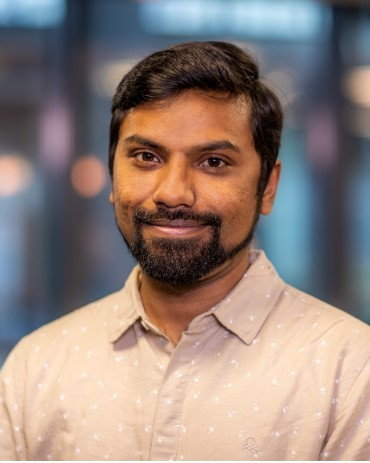
\includegraphics[width=0.35\textwidth]{Figures/sajid.jpg}
\end{wrapfigure}

% \begin{sloppypar}
Sajid Mohamed was born on July 6, 1990 in Trivandrum, Kerala, India. 
He studied at the National Institute of Technology (NIT) Calicut, where he obtained the Bachelor of Technology (B.Tech.) degree in Electrical \& Electronics Engineering in 2012.
He obtained his Master of Technology (M.Tech.) degree in Embedded Controls \& Software in 2014 from the Indian Institute of Technology (IIT) Kharagpur.
He was awarded the German Academic Exchange Service (DAAD) scholarship to pursue his Master's thesis
on Timed Abstractions and Analysis of Distributed Real-Time Control Architectures
at the Technical University of Munich (TUM) in the Institute for Real-Time Computer Systems.
He was a research assistant at IIT Kharagpur from 2014 to 2016.

In 2016, Sajid was awarded the Marie Skłodowska-Curie Scholarship and joined the Electronic Systems group of Eindhoven University of Technology (TU/e) as an Early-Stage Researcher in the \emph{Platform-aware Model-driven Optimization of Cyber-Physical Systems (oCPS)} project.
The project focused on training a generation of young researchers in cross-disciplinary thinking and delivering industrially validated toolchains by bringing together the state of the practice through six key industrial players and the state-of-the-art through four top universities and one research institute across Europe.
In 2020, Sajid continued working in TU/e as a University Researcher in the FitOptiVis project.
The results of his research have led, among others, to several peer-reviewed publications and the contents of this dissertation.
In July 2021, he started his current job as a Principal Software Engineer in the Innovation Team of ITEC B.V.
% \end{sloppypar}

\end{document}
